\documentclass{article}%
\usepackage[T1]{fontenc}%
\usepackage[utf8]{inputenc}%
\usepackage{lmodern}%
\usepackage{textcomp}%
\usepackage{lastpage}%
\usepackage{authblk}%
\usepackage{graphicx}%
%
\title{Differential regulation of Cu, Zn{-} and Mn{-}superoxide dismutases by retinoic acid in normal and psoriatic human fibroblasts}%
\author{Kevin Escobar}%
\affil{Department of Pediatrics and Molecular and Cellular Oncology, The University of Texas M. D. Anderson Cancer Center, Houston, TX, USA}%
\date{01{-}01{-}2014}%
%
\begin{document}%
\normalsize%
\maketitle%
\section{Abstract}%
\label{sec:Abstract}%
**UPDATE (1:05 p.m.) The E said that once activated, CREBH will activate several other genes that are associated with the cell's immune and inflammatory response in a variety of pathways in response to cancer. These include both alpha and beta {-} cell response enhancers, an umbrella term that includes both the DOT1 and C{-}reactive gene.**\newline%
Just what is terminal cancer meant to look like? Detecting the disease clearly isn't difficult in terms of a tumor finding, but how it develops is a bit different.\newline%
It is a human being with a terminal cancer genetic defect that, when passed on to a child, is able to cause late{-}stage cancer tumors that are able to grow through the destruction of the mutant cell proteins involved in cell regulation.\newline%
Normally, cancer detection relies on genetic screening to look for early{-}stage cancer that can have the potential to develop into non{-}tumor. In the case of terminal cancer, though, it starts with an otherwise healthy tumor.\newline%
That's where LTCs come in.\newline%
Enzymes in the digestive tract are the food and water proteins that help grow food and carry waste away from the body. LTCs are gene deletions and remissions of DNA that result in the cell shutting down its own immune system so it can't attack healthy cells.\newline%
"LTCs are replacing the gene functionality of the cells with another mutant or misfolded gene, which makes the cells less sensitive to defense, spreading faster," said Helen Deffine, MD, a professor of medical oncology at St. Jude Children's Research Hospital, who headed the research team that analyzed the evolution of c{-}reactive protein gene expression.\newline%
About a week after deffenmdine was able to detect the terminal cancer cell mutation in mice, she noticed that genetically similar tumors had been found in a team of human lTCs. The researchers concluded that c{-}reactive protein mutant has a devastating effect on cancer development.\newline%
DNA is regularly de{-}blanched to make an artificial expression of the gene while the cell is in response to it, stopping any production of c{-}reactive protein that would normally keep the cells in good shape. In a genotype in which c{-}reactive protein mutanting was detected while the LTCs{-}like mutation occurred, the genomes of the pro{-}survival lTCs were more misfolded and misdirected.\newline%
When genetic regions on the DNA were completely de{-}blanched, mutant, misfolded and misdirected, functional LTCs{-}like mutation arose even faster than normal stem cells in new tumors with no transition to normal cells.\newline%
When the tumors were treated by treating them with insulin, about 15 percent more C{-}reactive protein mutant gene expression occurred and tumors shrank by 40 percent to 45 percent.\newline%
"We're now able to identify the pathway that's causing these lTCs to disrupt and recreate an earlier outbreak of cancer. It's the missing puzzle piece to reverse progression. To make sure it doesn't happen again, we need to find the cells that produce it and reprogram them. It takes a pretty substantial investment, but if we can do it in a way that it doesn't take us away from treatment, patients won't have to be kept alive as long as they can, they will have a chance to live."\newline%
The research was published today in The International Journal of Clinical Oncology.

%
\subsection{Image Analysis}%
\label{subsec:ImageAnalysis}%


\begin{figure}[h!]%
\centering%
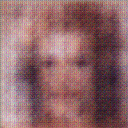
\includegraphics[width=150px]{500_fake_images/samples_5_110.png}%
\caption{A Close Up Of A Cat In A Room}%
\end{figure}

%
\end{document}